\chapter{Background} 
\label{cha:background}

In this chapter we provide some background on the topics relevant for this thesis. We begin by giving a general overview of software product lines, and continue by going into more detail on feature models and feature model evolution plans. Lastly, we give a short introduction to static analysis and its uses, as well as how it relates to the contributions of this thesis.

\section{Software Product Lines}
\label{sec:software-product-lines}

Software product lines (SPLs) are an engineering methodology used for developing products that share common features but have differences, for instance a product line of smartphones. When developing a software product line, engineers attempt to capitalize on the commonality by reusing components of source code for several of the products. For instance, all smartphones have technology for internet access. The final products of a software product line are called \emph{variants}, which consist of a combination of features available in the SPL. In a smartphone SPL, a variant is a complete smartphone. When software product lines were still a novel concept, engineers tended to throw together variants by copying and pasting the components where needed. When the SPLs grew larger, this process became increasingly error-prone. Each time a component needed to be updated, all variants using the component must be reviewed. In later years, however, several technologies have emerged that exploit the reuse of the components, combining the components together into a final product. This makes maintaining code  much more efficient and less error-prone, as each component only exists in one place.~\cite{book:introduction-to-spl}


\subsection{Feature Models}
\label{sub:feature-models}

\begin{figure}
   \begin{center}
      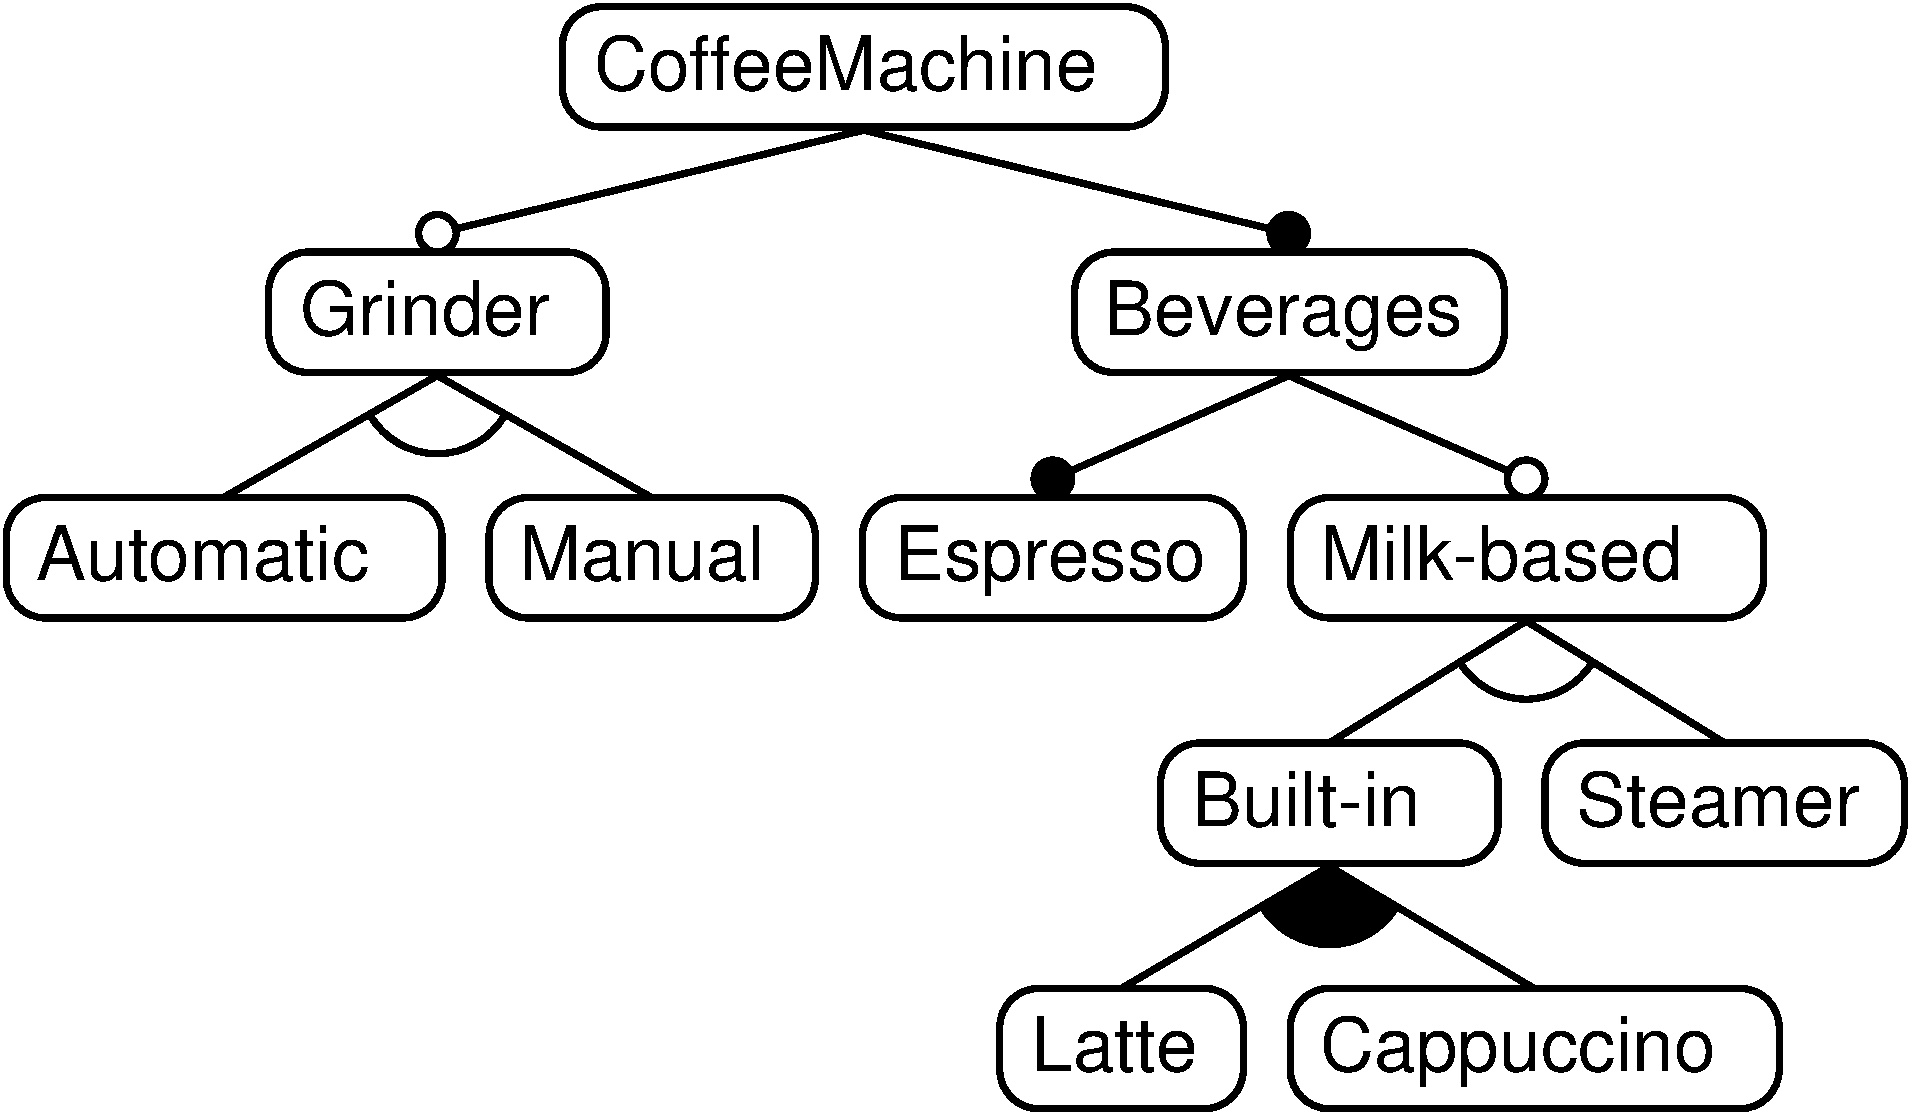
\includegraphics[width=0.6\textwidth]{CoffeeMachine1.pdf}
   \end{center}
   \caption[Example feature model for a coffee machine]{Example feature model for a coffee machine \protect\footnotemark}
   \label{ex:fm-coffee1}
\end{figure}
\footnotetext{Created using DarwinSPL: \url{https://gitlab.com/DarwinSPL/DarwinSPL}} %TODO: Move this to the correct page

\emph{Variability management} is the process of deciding which variants should be allowed, i.e. which combinations of features can be combined into a variant~\cite{art:variability-management-with-feature-models}. Formerly this was done as an informal process, often using spreadsheets and the engineers' intuition. To simplify and formalize this process we use \emph{feature models} to model the relations between the features (which combinations are allowed, which are common to all variants, etc.). Feature models can also be used as documentation for a SPL, providing a common language between stakeholders~\cite{book:introduction-to-spl}. A feature model is a tree-like structure where the nodes are features and groups of features. See Figure~\vref{ex:fm-coffee1} for an example of a feature model. A feature cannot be selected in a variant unless its parent feature is also selected~\cite{art:feature-models-grammars-and-propositional-formulas}.

A group gives logical structure to the features, restricting the allowed combinations of the features. For instance, in an \xortype{} group, exactly one of the features must be selected in every variant. In the example, the group under Grinder has this type. In a variant, a grinder cannot be both automatic and manual. Moreover, the features have types (\optional{} and \mandatory{}). A \mandatory{} feature must be selected in all variants, whereas an \optional{} feature may be left out. The black dot above Beverages means that this feature is mandatory, so all coffee machines provide beverages. Furthermore, since its child feature Espresso is also mandatory, all coffee machines have espresso. However, only some coffee machines have milk-based drinks, as shown by the white dot above the Milk-Based feature. If selected, then either built-in drinks such as latte or cappuccino must be included in the variant, or the machine must have a steamer so the user can make milk-based drinks themselves. The group under Built-in is filled-in with black, which means that it is an \ortype{} group. In a variant where Built-in is chosen, one or both of Latte and Cappuccino must also be chosen, but not zero. The groups which are neither \xortype{} nor \ortype{} have the type \andtype{}, which means that zero, one, or more of its child features may be selected in a variant. There are several restrictions to the structure of a feature model. For instance, an \xortype{} or \ortype{} group cannot contain a \mandatory{} feature. Although all features have a type, not all of them are displayed in this figure. The root feature (here CoffeeMachine) must have type \mandatory{}, since naturally it must be selected in all variants. Since an \xortype{} or \ortype{} group cannot contain a \mandatory{} feature, all features in those groups have the type \optional{}.

Feature models often also allow \emph{cross-tree constraints}. These are similar to the parent-child relation in the feature model but are independent of the tree structure. For instance, one could imagine that the producer would always include an automatic grinder if the Built-In feature is selected, because the built-in feature does not work unless the machine grinds the coffee automatically. This cross-tree constraint could be expressed as "Built-In requires Grinder``. Although cross-tree constraints are commonly used, we disregard them in this thesis. This is due to the fact that the cross-tree constraints add unwanted complexity, and we wish to exploit the tree structure of a feature model.

The formal structural requirements (well-formedness rules) to a feature model, as specified in~\cite{art:consistency-preserving-evolution-planning} are 
\begin{enumerate}[\itbf{WF\arabic*}, itemsep=0mm]
   \label{wf-requirements}
   \item A feature model has exactly one root feature.
   \item The root feature must be mandatory.
   \item Each feature has exactly one unique name, variation type and (potentially empty) collection of subgroups.
   \item Features are organized in groups that have exactly one variation type.
   \item Each feature, except for the root feature, must be part of exactly one group.
   \item Each group must have exactly one parent feature.
   \item Groups with types \xortype{} or \ortype{} must not contain \mandatory{} features.
\end{enumerate}

Furthermore, a feature model is a tree structure and must not contain cycles. There is an additional requirement that groups with types \xortype{} or \ortype{} must contain at least two child features, but this is not taken into account in this thesis. A \emph{paradox} is a violation of these well-formedness requirements, i.e. if the root is not mandatory, if a name is not unique, etc.

\subsection{Feature Model Evolution Plans}
\label{sub:feature-model-evolution-plans}
The evolution of an SPL can be planned using a \emph{feature model evolution plan}. Software product lines often grow very large, and it is crucial to plan ahead. 
There exist tools for evolution planning, such as DarwinSPL~\cite{art:darwinspl-an-integrated-tool-suite-for-modeling-evolving-context-aware-software-product-lines}. An intuitive way to think of an evolution plan is a sequence of feature models associated with the points in time when they are planned to be realized. For instance, imagine that the first coffee machines in the software product line are represented by the feature model in Figure~\vref{ex:fm-coffee1}. They are controlled by buttons, but as touch interfaces become more common, the manager decides to add coffee machines with a touch screen. This modification is included in Figure~\vref{ex:fm-coffee2}.


\begin{figure}
   \begin{center}
      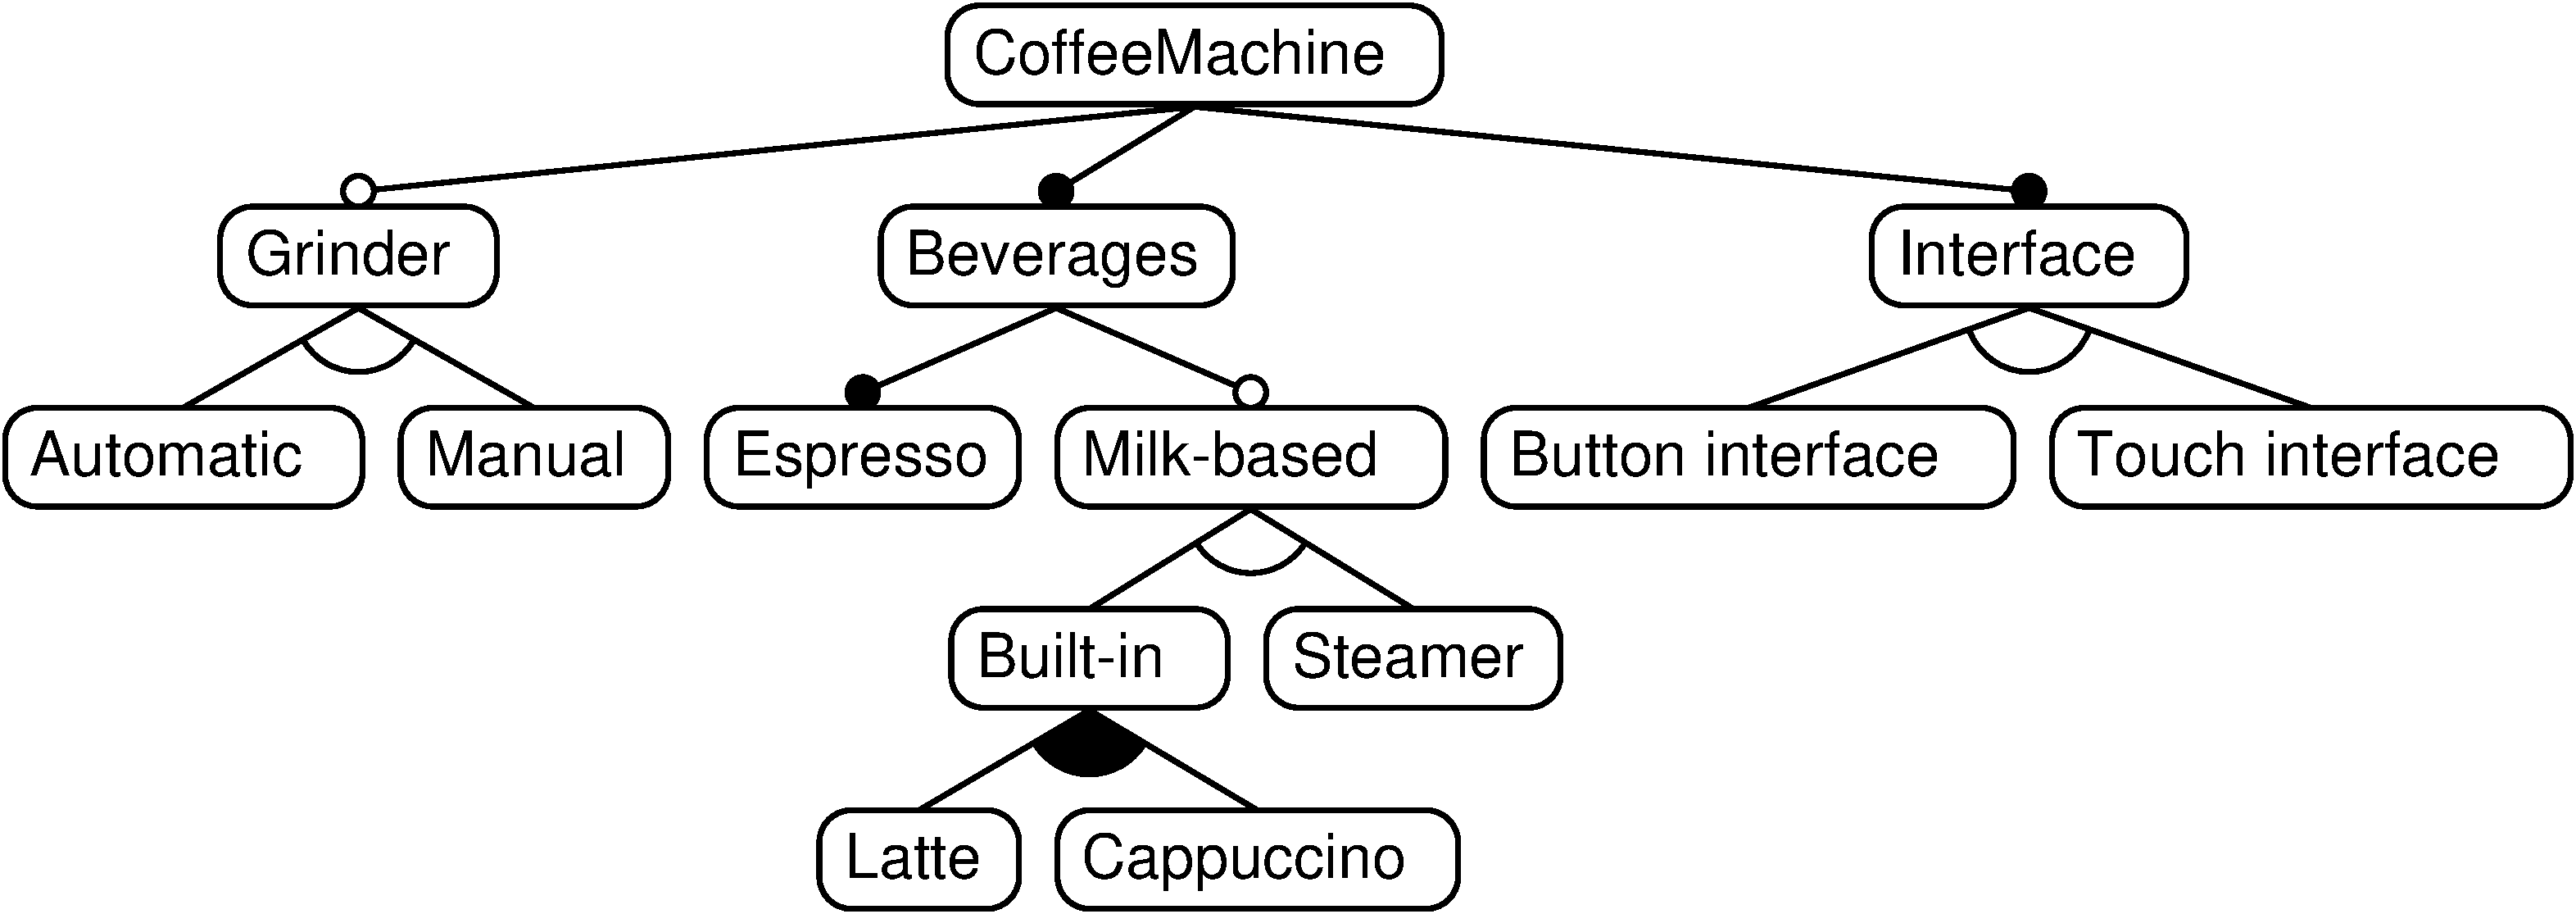
\includegraphics[width=0.9\textwidth]{CoffeeMachine2.pdf}
   \end{center}
   \caption[Coffee machine with added touch interface]{Coffee machine with added touch interface \footnotemark}
   \label{ex:fm-coffee2}
\end{figure}

\footnotetext{Created using DarwinSPL: \url{https://gitlab.com/DarwinSPL/DarwinSPL}} %TODO: Move this to the correct page

In the LTEP research project, we have formalized evolution plans as an initial model combined with a list of \emph{time points}, which are defined as points in time, associated with edit operations, e.g. change type of ``Beverages" to \optional{}. In the formalized feature model, each feature and group has a unique ID, and the edit operations use these IDs to uniquely identify the features and groups to be added, removed, or modified. To illustrate the idea, a simplified formalization of the evolution plan is shown in Figure~\vref{ex:formal-evolution-plan}. The initial model associated with time $t_0$ is the one shown in Figure~\vref{ex:fm-coffee1}. Applying the operations under $t_1$ results in the feature model shown in Figure~\vref{ex:fm-coffee2}. In the example, IDs are not used to improve readability, but in the formal definitions, such details are included in the operations and the feature model. 

\begin{figure}
   \footnotesize
   \begin{center}
      \begin{minipage}{0.98\textwidth}
         \begin{enumerate}[{\small $t_0$}]
            \item 
         \end{enumerate}
      \end{minipage}
      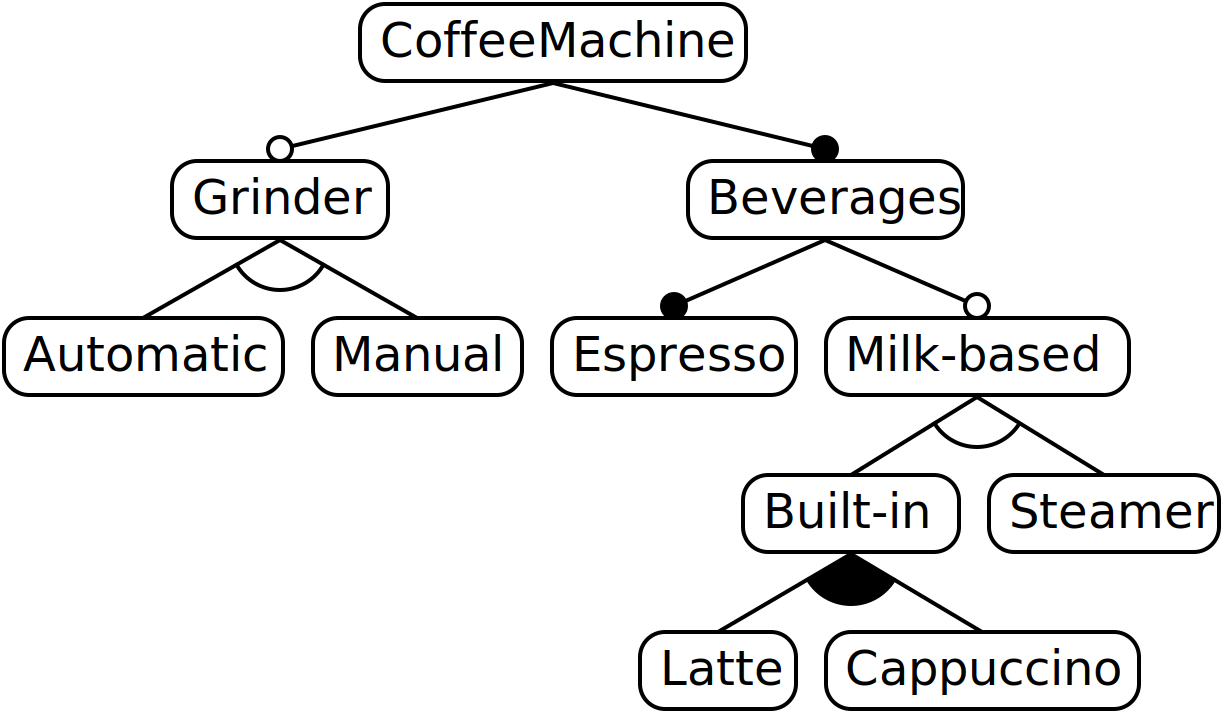
\includegraphics[width=0.7\textwidth]{CoffeeMachine1}
      \bigskip

      \begin{minipage}{0.98\textwidth}
         \begin{enumerate}[{\small $t_1$}]
            \item 
               \begin{enumerate}[ ]
                  \item Add new \mandatory{} feature ``Interface" to ``CoffeeMachine" \andtype{} group
                  \item Add new \xortype{} group to ``Interface"
                  \item Add new feature ``Button interface" to ``Interface" \xortype{} group
                  \item Add new feature ``Touch interface"  to ``Interface" \xortype{} group               \end{enumerate}
         \end{enumerate}
      \end{minipage}
      \caption{Formalized feature model evolution plan}
      \label{ex:formal-evolution-plan}
   \end{center}
\end{figure}

Furthermore, we have published a semantics for these edit operations along with a formal definition of a feature model, letting us define a \emph{sound} plan~\cite{art:consistency-preserving-evolution-planning}. The semantics is formalized as a set of structural operational semantic rules, detailing exactly which conditions must be fulfilled for an operation to be applied, and the way to construct the resulting feature model after applying it. A sound plan is an evolution plan in which applying each operation in order results in a structurally sound feature model for each step, i.e., a plan resulting in no paradoxes. Using this semantics on a modified plan allows for validation of change. When changing a feature model evolution plan, soundness of the updated plan can be checked by modifying the list of edit operations and checking that the resulting plan is sound using the semantics. However, this approach models change to \emph{feature models}, whereas the goal of this thesis is to model and analyse change to a \emph{feature model evolution plan}. 

\section{Static Analysis}
\label{sec:static-analysis}

Static analysis attempts to predict the behaviour of a program without executing it~\cite{book:principles-of-program-analysis}. This is different from \emph{dynamic} analysis, which analyses programs while executing~\cite{art:a-survey-on-static-analysis-and-model-checking}. Static analysis methods have various uses, including compilers, for instance for type checking, error detection~\cite{art:a-survey-on-automated-dynamic-malware-analysis-techniques-and-tools}, and optimizations; and lint tools, which detect possible errors the programmer is making while coding~\cite{art:industrial-perspective-on-static-analysis}. Furthermore, it is used to prove properties about programs, i.e. that the program behaviour matches the specification~\cite{art:a-survey-on-static-analysis-and-model-checking}. Due to the halting problem, an algorithm cannot in general decide exactly how a program behaves, but there exist several methods to safely approximate information. For instance, live variable analysis discovers which variables \emph{may} still be ``alive" (meaning used in the future) at a certain point of the program. Live variable analysis is done for optimization of memory allocation for variables. If a variable is known not to be live, it is safe to overwrite it with another variable. If a variable \emph{may} be live, it should not be overwritten. This makes live variable analysis a \emph{may analysis}. It is also a backward analysis since information about whether a variable is used in the future is carried backwards. There also exist \emph{must analyses} and \emph{forward analyses}. A must analysis looks for the greatest solution of things that \emph{must} be true. In a forward analysis, the information flows forward; meaning that what has happened earlier in the program influences the analysis at later points in the program~\cite{book:principles-of-program-analysis}.

Unlike programs, it is possible to get a full overview of a feature model evolution plan. It is always possible to find the correct answer given the question "Does feature A exist at time 5?". An operational representation finds the answer by applying operations to the initial model until time 5 is complete, and checks if feature A exists in the resulting feature model. For intuition on why this must be true, imagine a (correct) program where we know all statements are assignment. This program terminates for a certainty since there is no branching. The same goes for an operational feature model evolution plan. There are no conditional statements and thus no branching. Since we know that every operational feature model evolution plan ``terminates", we avoid the halting problem which is at the core of all static analysis of programs, which must always over- or under-approximate a solution to be certain that the analysis terminates.

May and must analyses always deal with \emph{scope}. When asking if a variable is live, we are also defining the scope of the variable, meaning which parts of the program the variable may be part of. Furthermore, the method for \emph{defining} the static program analyses can be applied to other domains. For instance, it is common to define these analyses in terms of rules on the form

\begin{prooftree}
   \AxiomC{$Conditions$}
   \UnaryInfC{$State \transition State'$}
\end{prooftree} 

where $State$ is the context when the rule is applied, and the $Conditions$ consists of propositions concerning the $State$. After the rule is applied, $State'$ is the result, usually a modified version of $State$. For instance, the semantics of an \textbf{if}-statement may be defined by the rules

\begin{minipage}{0.5\textwidth}
   \footnotesize
\begin{prooftree}
   \AxiomC{$\lookup{\Gamma}{b} = \top $}
   \RightLabel{$\textsc{If}_1$}
   \UnaryInfC{$\langle \Gamma, \, \textbf{ if } b \textbf{ then } S \textbf{ else } S' \rangle \transition \langle \Gamma ,\, S \rangle$}
\end{prooftree}
\end{minipage}
\begin{minipage}{0.5\textwidth}
   \footnotesize
\begin{prooftree}
   \AxiomC{$\lookup{\Gamma}{b} = \bot $}
   \RightLabel{$\textsc{If}_2$}
   \UnaryInfC{$\langle \Gamma, \, \textbf{ if } b \textbf{ then } S \textbf{ else } S' \rangle \transition \langle \Gamma ,\, S' \rangle$}
\end{prooftree}
\end{minipage}

Here, $\Gamma$ is the context treated as a map from variable names to values, and $\lookup{\Gamma}{b}$ returns the value of $b$ at the time when the statement is executed, which is either $\top$ (true) or $\bot$ (false). If the expression $b$ is true, then the next statement to be executed is $S$. If not, then the next statement is $S'$. Notice that no rule defines the program behaviour if the value of $b$ is neither $\top$ nor $\bot$. This means that anything other than $\top$ or $\bot$ is an error, and an implementation of the language will provide an error message for such a case. This is a useful property of these rules, as there are often many ways to write an incorrect program, and all of these can be captured by \emph{not} fitting the correct cases.

The syntax-driven, unambiguous, and compact nature of such rules make them popular for formally defining type systems and analysis tools~\cite{book:principles-of-program-analysis}. Here, they give both the behaviour of the if-statement (semantics) using the syntax of the language, and, implicitly, they provide a method for checking correctness of an if-statement. If the expression is neither true nor false, then the program is incorrect. In this thesis, we largely exploit this property of only defining the correct cases when giving rules for soundness analysis of modifying feature model evolution plans.

% Give static analysis \emph{way of thinking} as background, not the exact methods used to analyse programs, but the principles such as may/must analysis etc. Explain how it is communicated (rules), how scope is a factor and discuss soundness in static analysis context (this is the same as the soundness I talk about). 


% Static analysis is semantic-based analysis. Syntax-driven, but semantic-based, but also of the meaning. If we have x := 5, then it means that 5 is the value which you put into x
% Say that I'm doing semantic-based analysis in the thesis, _analysis_, not just semantics.Can I add it or not? How much of the scope is affected? Emphasize modularity; analysis is modular. Focus on the analytical parts of the work, combined with the semantics of a feature model
% Don't call the rules SOS rules, but "Rules for semantics-based analysis". Stop downplaying
% Give the structure of the rules in the background. Static analysis has an environment and an effect. I'm making a calculus
% Analysis is formalized through a set of rules, which often have this kind of structure... which also looks very much like SOS rules.
% Emphasize that I've made an implementation as well as the theory.
\subsection{Soundness}
A feature model evolution plan may be viewed as a sequence of feature models associated with time points. 
In this context, soundness of a feature model evolution plan means that all of the feature models in the plan uphold the structural requirements \itbf{WF1\textendash WF7} given in Section~\vref{wf-requirements}. In a sound plan, no paradoxes occur; for instance, no two features have the same name at the same time, no groups with type \xortype{} or \ortype{} contain features of type \mandatory{}, etc. This can be verified automatically, as we did in \cite{art:consistency-preserving-evolution-planning}.
